\documentclass[acmsmall,nonacm,natbib=false]{acmart}

\usepackage{graphicx}
\usepackage{booktabs}
\usepackage{amsmath}
\usepackage{float}
\usepackage{multirow}
\usepackage{array}
\usepackage{xcolor}
\usepackage{hyperref}
\usepackage{fontawesome5}
\usepackage{wrapfig}

\newcommand{\githublink}[2]{\href{#1}{\faGithub\ #2}}

\AtBeginDocument{%
  \providecommand\BibTeX{{Bib\TeX}}}

\settopmatter{printacmref=false}
\renewcommand\footnotetextcopyrightpermission[1]{}
\setcopyright{none}

% ===== Margin Adjustments =====
\setlength{\topmargin}{-0.6in}
\setlength{\textheight}{8.9in}

\setlength{\oddsidemargin}{-0.45in}
\setlength{\evensidemargin}{-0.49in}
\setlength{\textwidth}{5.7in}

\setlength{\headheight}{8pt}
\setlength{\headsep}{8pt}



\begin{document}


% =================================================
% COVER PAGE
% =================================================
\begin{titlepage}
    \centering
    \vspace*{2cm}

    {\Huge \textbf{Network Data Analysis Coursework}\par}
    \vspace{1.5cm}

    {\large Submitted by\par}
    \vspace{0.3cm}
    {\Large Gayathri Ganeshan Nair\par}
    \vspace{0.5cm}

    {\large K-number: K25038453\par}
    \vspace{0.5cm}

    {\large King's College London\par}
    \vspace{1cm}

    {\large Repository Link:\par}
    \vspace{0.3cm}
    {\normalsize \url{https://github.kcl.ac.uk/k25038453/network-data-analysis-coursework}\par}

    
\end{titlepage}


% =================================================
% MAIN REPORT
% =================================================

% The coursework consists of 2 parts, which are about Wikidata Editor Networks and the Leeds Road Network and Accident Analysis.\\

% =================================================
% PART 1
% =================================================

\section{\LARGE{Part 1: Wikidata Editor Networks}}


\subsection{\large{Data Selection and Preprocessing}}

Part 1 uses datasets from the Wikidata Talk page that show how editors interact with each other. Three datasets were chosen based on the size of the files, which was used as a stand-in for the size of the network: REQUEST\_FOR\_DELETION (large), USERS (medium), and REQUEST\_A\_QUERY (small). There are three columns in each dataset:
username, thread\_subject, and page\_name. Before building the network, rows with missing values were taken out, and string fields were made more consistent by cutting out extra spaces. The same preprocessing pipeline was used on all three datasets, but they were kept as separate networks.


\subsection{\LARGE{Task A: Network Construction}}

 This task turns each Wikidata discussion dataset into an editor interaction network, where users are linked by their shared involvement in the same discussion. To make sure that the modelling was the same and that the results could be compared, all the datasets used the same construction pipeline. Undirected graphs were used because co-participation in the same thread does not imply an observable
reply direction. The implementation is provided in \githublink{https://github.kcl.ac.uk/k25038453/network-data-analysis-coursework/blob/main/notebooks/part\_1/taskA.ipynb}.


\subsubsection{\large{\textbf{"What elements of the dataset you represented as nodes and edges?"}}}
\leavevmode \par \noindent
Nodes represent the Wikidata Editors, identified by \textit{username} attribute. Edges represent the social connections/interactions among the users who made comments within the same \textit{thread\_subject} and the same \textit{page\_name}. This produces an undirected interaction graph in which shared participation is used as a proxy for conversational interaction.  
This abstraction adheres to the graph-modelling perspective examined in the module, wherein the network encapsulates entities and their interrelations while extraneous details are omitted \cite{easley2010networks}.
A preliminary visual examination of the constructed graphs (Appendix~\ref{appendix:visuals}) corroborates this modelling decision by illustrating clustered interaction structures instead of discrete pairwise reply links \cite{newman2010networks, easley2010networks}.

\subsubsection{\large{\textbf{"What data structures did you choose to represent this network? How do you keep additional information that cannot be directly encoded as nodes and edges? "}}}
\leavevmode \par \noindent
Different data structures were used at different stages of the implementation. In the beginning, the dataset was loaded into a \textit{pandas dataframe}, which provided the tabular structure for cleaning the data, reviewing the rows, and grouping interactions by \textit{page\_name} and \textit{thread\_subject}. The structure was useful as the original data was relational, but not in graph form yet. Python dictionaries were used to organise the workflows across the three selected datasets. One used to store the dataset file paths, while another stored constructed graphs indexed by dataset size. This enabled us to apply the same processing pipeline consistently across all the datasets.\\
The final network in itself was represented using a \textit{NetworkX undirected graph}, in which, each user corresponds to a node, and an edge is added between two users if they commented in the same thread on the same page. This way it is better for modelling social interaction as it supports standard network operations like counting nodes and edges, identifying connected components, and computing graph metrics  \cite{hagberg2008exploring, newman2010networks}.\\
Additional information, such as \textit{page\_name} and \textit{thread\_subject}, was not directly encoded as separate nodes or edges in the final graph. Instead, it was retained in the dataframe during preprocessing and grouping, where it served as the contextual information for defining interactions.
In network modelling, it is common to keep attributes separate from the main topology \cite{newman2010networks}.
Numeric identification was not needed because NetworkX can use usernames as node identifiers without changing their uniqueness.



\subsubsection{\large{\textbf{"What was your algorithmic approach for building the network?"}}}
\leavevmode \par \noindent
We made the network by turning the tabular interaction data into a graph. In this process, we have followed a grouping-based approach to discover any relations between the users, depending on their presence in the same discussion. Firstly, each dataset is preprocessed by filtering out the missing rows in addition to normalising the strings for \textit{username, thread\_subject}, and \textit{page\_name} attributes. The cleaned data is grouped by the pair \((\textit{page\_name}, \textit{thread\_subject})\), so that each group corresponds to one unique discussion context.\\
All unique users within each group are first identified. Then, edges are created using all combinations of user pairs, in any order, in each group. In the case of \( (u_i, u_j) \), an undirected edge is added to the graph, meaning that the two users have co-participated in the discussion together. The results show that a clique is formed in each group of discussions. In order to guarantee computational efficiency while dealing with big data, a restriction is imposed to minimise the number of users taken into account within very large forums. This reduces the risk of excessive edge generation in usually large discussion groups, while having a limited effect on the broader construction logic.\\
It should be noted that this type of modelling technique follows traditional graph computational models where the relationship is created based on shared context instead of direct interaction between two people \cite{newman2010networks}. Moreover, creating groups and connecting individuals based on shared context seems similar to affiliation networks where individuals are connected due to their involvement in specific events \cite{easley2010networks}.\\
We chose the above option because the dataset doesn't have clear reply or timestamp information.
So, other models that use directed edges or temporal interactions would need information that isn't in the source data. So, this model gives a fair picture of how people interact with each other based on the assumptions made. We also looked at the networks we built (Appendix~\ref{appendix:visuals}). Because the graphs were different sizes, the small dataset was shown in full, while the medium and large datasets were only shown with representative subgraphs and the biggest connected components. The small graph has one main connected component that makes up most of the graph, while the medium and large graphs have a dense core with a lot of peripheral clusters. These patterns are consistent with connected-component statistics and the common characteristics of real-world social networks \cite{newman2010networks, watts1998collective, easley2010networks}. The implementation is still flexible because you can make different network definitions by changing the grouping columns and user ID.



\subsection{\LARGE{Task B: Network Metrics}}
\leavevmode \par \noindent
This task analyses the constructed Wikidata editor networks using structural metrics and comparison with random graphs. The objective is to characterise their properties and position them within the regular–small-world–random network spectrum. The implementation is provided in \githublink{https://github.kcl.ac.uk/k25038453/network-data-analysis-coursework/blob/main/notebooks/part\_1/taskB.ipynb}.

\subsubsection{\large{\textbf{"What are the characteristic properties and relevant metrics and distributions of this Wikidata editor network?"}}}
\leavevmode \par \noindent
The three Wikidata editor networks were analysed using standard structural metrics, including network size, density, average degree, clustering coefficient, size of the largest connected component, and path-based measures computed on the largest connected component. Results related to the analysis of these metrics are listed in Appendix~\ref{appendix:taskB_basic} and Appendix~\ref{appendix:taskB_path}. \\
All three datasets are sparse, with density decreasing as network size increases. At the same time, the average degree is relatively constant for all three networks, which implies that users' behaviour does not change depending on network size. Such behaviour is commonly observed in large-scale social networks, where local interaction rules remain consistent even as the system grows \cite{newman2010networks}.\\
Each network contains a dominant giant connected component, showing that most of the users are connected to one another indirectly through their common discussion contexts. However, it is observed that the degree of fragmentation varies for each dataset, with the medium-sized network exhibiting a larger number of disconnected components compared to the small and large networks. This implies that cohesion is dependent upon both the size and content of discussion activities in each network.\\
Clustering coefficients are high in all three networks.  This signifies that users participating in the same discussion tend to form tightly connected groups, which is consistent with social interaction patterns where shared contexts lead to increased likelihood of connection.\\
The degree distributions in Appendix~\ref{appendix:degree_distribution} show a heavy-tailed pattern, with many low-connectivity users and a small number of highly connected hubs. This unequal distribution of interactions is characteristic of real-world communication networks \cite{newman2010networks}.\\
Finally, path-based metrics indicate that the networks maintain relatively short average path lengths and small diameters, implying efficient connectivity within the largest connected component. This suggests that information or interaction can propagate across the network with relatively few intermediate steps.

\subsubsection{\large{\textbf{"How different is this network from a random network, according to the various comparison criteria we have seen in class?"}}}
\leavevmode \par \noindent
The structural differences between the Wikidata editor networks and random networks were evaluated using Erd\H{o}s--R\'enyi (ER)  graphs having the same number of nodes and similar edge densities. In such random networks, edges are formed independently with probability \(p\), leading to binomial (or approximately Poisson) degree distributions and low clustering coefficients \cite{easley2010networks,newman2010networks}.\\
An important difference is the higher level of clustering in the real-world graphs compared to their random counterparts (refer to Appendix B, Appendix~\ref{appendix:taskB_random} in particular). In other words, edges do not form randomly, but instead they tend to appear locally in groups. Such observation corresponds to the idea of triadic closure introduced in the module, which implies the existence of mutual ties among users participating in the same discussion context \cite{easley2010networks}.\\
The degree distributions for Wikidata networks differ significantly from those for ER model random graphs. While random graphs produce narrowly concentrated degree distributions around the mean, the Wikidata networks display heavy-tailed distributions (Appendix~\ref{appendix:taskB_figures}), indicating the presence of highly connected nodes alongside many low-degree users. Thus, the distribution of the interaction within such networks is uneven, implying that a few nodes will dominate interactions.\\
Regarding path lengths, real networks exhibit short average path lengths alongside high clustering coefficients. Conversely, random networks display average path lengths but low clustering coefficients. As discussed in the module, this combination is not characteristic of random graphs but instead defines small-world networks \cite{watts1998collective,milgram1967smallworld}.\\
In summary, Wikidata networks can be said to differ from random networks in that their social structure is reflected in their connectivity rather than random link formation. The simultaneous presence of high clustering, heavy-tailed degree distributions, and short path lengths make them fit into the category of small-world networks.

\subsubsection{\large{\textbf{"If you take this network as a complete and representative description of editor networks in collaborative knowledge projects like Wikipedia and Wikidata, what does it tell you about the way editors talk among themselves and their social activity and connections?"}}}
\leavevmode \par \noindent
Considering the structural characteristics of the editor networks of the Wikidata, it can be seen that the editor interaction is not randomly distributed and uniform, but rather organised by means of interplay between local clustering and global connectivity. High values of clustering coefficients imply that the users tend to belong to tightly connected clusters which correspond to discussions on the same topics/pages. This is related to the assumption that the shared context fosters the development of interaction among the users, which is in line with the affiliation networks approach \cite{easley2010networks}.\\
At the same time, the presence of a dominant giant connected component across all datasets implies that these local groups are not isolated, but are indirectly connected through shared participants. Combined with short average path lengths, this indicates that the network supports efficient communication across the broader system, even though interactions primarily occur within smaller communities.\\
The heavy-tailed degree distributions (Appendix~\ref{appendix:taskB_figures}) further reveal that editor activity is highly unequal. A vast majority of users participate in only a small number of discussions, while a relatively small subset of users is highly connected and likely functions as hub nodes linking together different discussion groups. These users play an important structural role in maintaining overall connectivity and facilitating the flow of information across the network.\\
The differences between the three datasets are driven more by interaction structure and discussion
context than by network size alone. Some discussion contexts might allow more dispersed and disconnected interactions, whereas in other environments, interactions might be more connected and integrated.
Overall, these findings imply that collaborative knowledge platforms such as Wikidata operate through a balance of local group interactions and global connectivity, supported by structurally important users who link communities. Such a model of operation is consistent with large social networks in general and is consistent with the activity patterns observed in them \cite{leskovec2008planetary,newman2010networks}.



\subsection{\LARGE{Task C: Epidemic Models}}
This task aims at understanding how suspicious or controversial behaviour may propagate through Wikidata editor networks using network-based modelling approaches. The purpose is to understand the plausibility of such behaviour to remain localised and identify effective strategies for selecting the editors to monitor. This approach involves the application of shortest-path measures, local neighbourhood structures, and epidemic-style diffusion models. The code implementation is available from \githublink{https://github.kcl.ac.uk/k25038453/network-data-analysis-coursework/blob/main/notebooks/part\_1/taskC.ipynb}.

\subsubsection{\large\textbf{{"If both editors have been commenting more than usual on the same day (i.e. might be controversial, trolling, etc.), how can they use the network data to judge how plausible it is that this behaviour has not propagated yet to neighbouring similar editors?"}}}
\leavevmode \par \noindent
The plausibility of non-propagation can be assessed by analysing the local structural position of the suspicious editors as well as their exposure to spreading effects through an evaluation of the susceptibility of their neighbouring nodes. This is assessed using the shortest-path distance and the local network structure. From a network point of view,  if suspicious editors are embedded in densely connected regions with many immediate neighbours and overlapping connections, then there exist multiple pathways through which behaviour could propagate. Alternatively, if the suspicious editors reside in loosely connected regions or have limited interaction overlap with other nodes, the assumption of non-propagation becomes reasonable.\\
For this purpose, the study focuses on two measures related to the size of the immediate neighbourhood (1-hop neighbours) and the size of the extended neighbourhood (2-hop nodes), along with a degree of structural similarity between editors through the examination of shared neighbours. The greater number of neighbours and common neighbours indicate stronger local connectivity and greater opportunities for propagation. This aligns with the concept of triadic closure, where individuals connected to the same neighbours are more likely to become connected themselves, reinforcing local clustering and facilitating spread \cite{easley2010networks}.\\
The existence of shorter paths provides an alternative perspective in that it demonstrates how rapidly the information or behaviour can diffuse into other regions of the network. When the nodes are clustered closer around the suspicious editors, the whole network can be reached swiftly, leading to a low likelihood of non-propagation. This phenomenon aligns with the small-world property found in many real networks due to its short path lengths \cite{watts1998collective,milgram1967smallworld}.\\
Plausibility indicators calculated from the two datasets (neighbourhood size and similarity) are described in Appendix~\ref{appendix:taskC_plausibility}. It is shown that the more connected the neighbourhoods are within the networks, the structural conditions favour propagation, thereby reducing the plausibility that suspicious behaviour remains isolated. Networks can be used in evaluating non-propagation by using density, structural similarity, and reachability indicators, taking into account immediate exposure of neighbouring editors and possible propagation, allowing the Wikimedia Foundation to make informed judgements about whether suspicious activity is likely to have already propagated.

\subsubsection{\large\textbf{{"If one or both of the tested editors have indeed been “possibly trolling”, then the Foundation will start checking other editors as well, prioritising those with a higher chance of having been trolling. How should they use the data to come up with a priority list on what editors to check first?"}}}
\leavevmode \par \noindent
The prioritisation problem can be approached by combining multiple network-based signals instead of focusing on one. In this work, suspicious editors are ranked according to three different criteria:\-\\
1. The first criterion is structural proximity, i.e., the shortest path distance to suspicious editors. Editors closer to suspicious editors, according to shortest paths, should be checked first since they have a greater chance to come in contact with the suspicious behaviour along the chain of interactions. Thus, shortest paths serve as a good measure for assessing how fast suspicious behaviours could propagate through the network. Such consideration is especially important in small-world networks, where short paths could help propagate information even in very large networks \cite{watts1998collective,milgram1967smallworld}.\\
2. The second criterion is local similarity and exposure. Editors connected to suspicious editors or having many neighbours in common with suspicious editors should be evaluated further. From a network perspective, this approach is aligned with triadic closure and affiliation-based interaction, where users participating in common local contexts are more likely to become structurally connected and to influence one another \cite{easley2010networks}. Thus, local overlap helps identify editors who are not just close in distance, but embedded in the same interaction environment.\\
3. The third criterion is repeated reachability under a diffusion process. For the purposes of estimation, a simplified epidemic-style simulation was carried out to approximate the probability of the editor being reached, allowing for suspicious activity to spread probabilistically from the intial seed users. By running multiple iterations of the algorithm, one obtains a more stable estimation of which editors would repeatedly become reached, assuming the diffusion assumption holds.  In such a case, repeated reachability of the editor suggests a vulnerability to a broader range of spreading processes, implying greater prioritisation in the context of our analysis. This adheres to the intuition behind epidemic and cascades models learned during the module, where the ability to spread does not just depend on distance but also on local branching opportunity and repeated exposure \cite{easley2010networks}.\\
These three rankings are then combined into a final priority score. Editors ranked highly across multiple methods are treated as stronger candidates than editors highlighted by only one criterion.  This way of prioritising the candidates is preferable to the degree-based ranking as discussed above. Indeed, the approach based solely on the degree criterion risks over-prioritising redundant or non-vulnerable nodes, even if they happen to be very popular.  According to the materials covered during the module on influence maximisation, such an approach could be inefficient when dealing with structurally overlapping nodes being repeatedly chosed  discounting or combining information across local structures can produce better prioritisation strategies \cite{easley2010networks}.\\
If only one editor is suspicious, it will be important to give high priority to those nodes that are located nearby and within the nearest network neighbourhood of the suspicious node. In case of two suspicious editors, preference should be given to those nodes that are close to both suspicious editors, shared by the network neighbourhoods of suspicious nodes, or reached by using both as seeds in simulations. Simply put, two suspicious nodes can strengthen a particular local community or provide several possible points of entry into the network, thus requiring immediate action.
The resulting combined rankings and one-seed versus two-seed comparisons are reported in Appendix~\ref{appendix:taskC_priority}. As a result, we propose that prioritisation is based on the joint consideration of several centrality metrics, including distance, similarity in the local neighbourhood, and exposure to information diffusion, giving the Wikimedia Foundation a solid basis for choosing those editors to investigate first.


\subsection{\LARGE{Comparative Discussion Across the Three Selected Networks}}

\subsubsection{\textbf{\Large{Similarities}}}
\leavevmode \par \noindent
All three networks are characterised by being sparsely connected and contain a huge single giant connected component (Appendix~\ref{appendix:A.2} and Appendix~\ref{appendix:B.1}). Despite the differences in size, the average degree is more or less stable, which implies that the interaction behaviour did not vary much from one case to another. All three networks additionally showed a combination of high clustering with short path lengths (Appendix~\ref{appendix:B.2}), and similar properties were identified during the propagation task since the behaviour could travel through a significant part of the network in just a few moves (Appendix~\ref{appendix:C.3}).\\
By analysing degree distributions plots (Appendix~\ref{appendix:B.4}) for all three networks, heavy-tailed patterns were detected in each case, implying that a small number of highly connected editors serve to maintain the connectivity of the network. This was further observed in Task C, where propagation and prioritisation pointed to important structurally central nodes as potentially dangerous options (see implementation: \githublink{https://github.kcl.ac.uk/k25038453/network-data-analysis-coursework/blob/main/notebooks/part\_1/taskC.ipynb}). Summarizing all findings, we can claim that all three networks functioned similarly, in terms of structural efficiency and propagation capability, positioning them within the small-world area of the network spectrum.

\subsubsection{\textbf{\Large{Differences}}}
\leavevmode \par \noindent
Despite the similarity in the overall structural arrangement, the datasets vary in the internal connectivity of the graphs. For example, the small network is very cohesive because most nodes belong to the largest connected component (Appendix~\ref{appendix:B.1}). Similarly, the propagation behaviour in Task C is fast and dense due to the existence of many densely connected local neighbourhoods (Appendix~\ref{appendix:C.1}).\\
On the other hand, the medium network is more fragmented, with many disconnected components (Appendix~\ref{appendix:A.2}). This separation in the network structure directly translates into a non-uniform and locally focused propagation behaviour, which is supported by a high average shortest path length and diameter (Appendix~\ref{appendix:B.2}).  Information diffusion in the medium network needs to follow more hops, making it harder for the information to spread compared to the other networks.\\
The large network has a similar level of connectivity to the small network, except that the latter network has a highly distributed structure, i.e. the largest connected component is massive and has a great reach (Appendix~\ref{appendix:C.3}). The propagation results show that behaviour spreads widely even from a small number of seeds, highlighting stronger global connectivity. These differences demonstrate that propagation behaviour is influenced more by structural organisation than by network size alone.

\subsubsection{\textbf{\Large{Effect of Modelling Choices}}}
\leavevmode \par \noindent
Network properties and propagation phenomena depend heavily on the way the network is modelled for Task A. Creating edges between individuals who participate in a discussion implies that the network will necessarily contain a large number of densely connected clusters of nodes, thus increasing the clustering coefficient values for all datasets (Appendix~\ref{appendix:B.1}). This modelling method enhances local connectivity and raises the chances for propagation to occur, especially in the case of densely connected clusters in Task C.\\
Furthermore, considering the graph as undirected makes interaction simpler by implicitly accepting that users mutually influence each other, despite no information regarding the direction and timing of replies being provided in the initial dataset. This may result in an overestimate of the propagation capability of the network, especially when simulating diffusion (Appendix~\ref{appendix:C.3}). The constraint applied on group sizes also changes the network properties by decreasing its tendency to form very connected nodes, making hubs less dominant in the network while remaining computationally feasible (implementation: \githublink{https://github.kcl.ac.uk/k25038453/network-data-analysis-coursework/blob/main/notebooks/part\_1/taskA.ipynb}).\\ 
As such, the observed networks tend to resemble small-world networks more rather than completely random or regular networks due to the presence of both high clustering coefficients and short average shortest paths (Appendix~\ref{appendix:B.3}). However, this positioning is partly shaped by the modelling assumptions, particularly the clique-based construction, which enhances local clustering and influences the observed propagation behaviour.



% =================================================
% PART 2
% =================================================

% make sure to put


\section{\LARGE{Part 2: Leeds Road Network and Accident Analysis}}

%The dataset does not contain explicit geographic coordinates; therefore, the study area is selected based on inferred high-activity regions rather than exact spatial filtering.


\subsection{\large{Study Area and Data Sources}}
\leavevmode \par \noindent
This coursework part two involves spatial network analysis of a road network and any events related to it, located in Leeds, United Kingdom. A network-based approach to analysing spatial events has been used, wherein roads represent the edges and the junctions the nodes, while processes occurring on the network are considered instead of an open plane space. This approach satisfies the basic premise of spatial network analysis in which measurements take place along the network itself instead of Euclidean distance measure \cite{okabe2000spatial}.\\
Road network for the city of Leeds was taken from the OpenStreetMap data using the OSMnx library, which provides a facility for acquiring, constructing and analyzing street networks as graphs \cite{boeing2017osmnx}. Only roads accessible to vehicles were considered to ensure relevance to our problem of road traffic accidents, as spatial analysis of networks depends heavily on their graph properties; inclusion of other paths would affect measures of connectivity, density and route length, etc.\\
The road accident data was obtained from the United Kingdom Government’s open data website, which contains extensive information about traffic accidents. Road accident datasets from 2014, 2015, and 2016 were merged into a multivariable dataset. The use of multiple years allows for a more stable analysis process by reducing the influence of short-term fluctuations and providing a more representative view of accident patterns. A fixed research area of about 1 km$^2$ was chosen in central Leeds to provide uniformity in the research process. The choice of the research area was made based on spatial centrality and accident density to focus on the most active area in terms of statistics. The search area was limited to a central Leeds window containing the median of all accident locations, meaning that the final research area is both spatially central and highly accident concentrated.\\
The spatial information was expressed through a projected coordinate reference system because distance and area calculations require such data. It is necessary for solving problems related to shortest paths, edge length, and spatial statistics that imply using metric rather than angular coordinates.\\
Tasks of Part 2 are based on the same common dataset and network representation.  Task A focuses on structural properties of the road network, Task B investigates accident patterns as events occurring on the network, and  Task C uses ideas of network partitioning and routing for solving the problem of organising marathons in the city. Together, these tasks demonstrate how concepts from graph theory and spatial network analysis can be applied to real-world urban systems \cite{easley2010networks}.

\subsection{\LARGE{Task A: Spatial Networks and Planarity}}
\leavevmode \par \noindent
This task will involves the construction of a drivable road network for an area in central Leeds using data from OpenStreetMaps along with several years' worth of accident statistics. In accordance with the requirements of the coursework, the study area was selected to be about 1 km$^2$ in size and having many accidents per year. Following the principles of spatial network analysis that were covered in this module, the road network is modelled as an edge graph with nodes at intersections, and distances are measured along the network rather than in unrestricted planar space \cite{okabe2000spatial,boeing2017osmnx}.  The implementation is provided in the accompanying repository \githublink{https://github.kcl.ac.uk/k25038453/network-data-analysis-coursework/blob/main/notebooks/part\_2/taskA.ipynb}.




\subsubsection{\large\textbf{{"What are the coordinates of the chosen area?"}}} 
\leavevmode \par \noindent
The selected study area was taken to be a 1 km$\times$1 km square situated in central Leeds. In order to validate this selection, accident data for the years 2014--2016 were aggregated into point geometries and transformed into the British National Grid coordinate system. Next, a moving window analysis was performed using a central Leeds search window that was based on the median location of accidents. 
\begin{wrapfigure}{l}{0.45\textwidth}
    \centering
    \vspace{-10pt}
    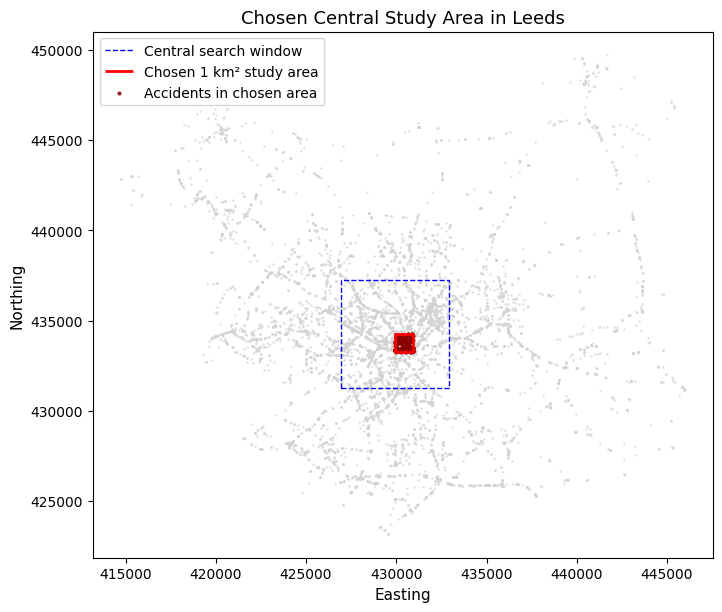
\includegraphics[width=0.4\textwidth]{figures/taskA_area_selection.png}
    \caption{Selection of the final 1 km$^2$ study area in central Leeds.}
    \label{fig:taskA_area_selection}
    \vspace{-10pt}
\end{wrapfigure}
Only central Leeds windows around the median accident location were considered; thus, the final selected 1 km$^2$ square is not only central but also accident-heavy. This procedure identified the candidate square containing the highest multi-year accident count within the central search region.
The total number of accidents within the selected 1 km$^2$ square over three years is 313, which meets the coursework criteria of choosing an area with a considerable number of accidents. Coordinates of the selected area are:\\
\textbf{Easting: 429934 to 430934}\\
\textbf{Northing: 433255 to 434255} \\
Coordinates of the chosen box are approximately $(53.79923, -1.53943)$ latitude and longitude respectively. Procedure for choosing the study area is presented on Fig.~\ref{fig:taskA_area_selection}. Accident distribution in the entire city, used as an incentive for searching in the centre of the city, is presented in Appendix~\ref{appendix:part2taskA_q1}.



\subsubsection{\large\textbf{{"What are the characteristics of this road network? Include, at least, the spatial diameter of the network, the average street length, node density, intersection density, and edge density."}}} 
\leavevmode \par \noindent
The road network data of the selected study area was obtained from OpenStreetMap with OSMnx \cite{boeing2017osmnx}. In accordance with the instructions in the coursework, only the drivable roads have been selected based on the drivable street network data, and not the pedestrian paths. The selection criterion of \texttt{network\_type='drive'} ensures that the roads selected are those meant to be driven and can thus be considered as suitable for road traffic analysis.
After conversion into the metric coordinate system, the extracted drivable road network consists of 204 nodes and 347 edges. Calculation of standard street-network statistics with OSMnx, similar to how spatial road networks are treated in the module, involves the calculation of statistics like average street length, node density, intersection density, and edge density of the graph \cite{boeing2017osmnx}. Calculations of the weighted spatial diameter have been carried out using shortest-path distances between pairs of nodes with weights corresponding to edge lengths, as the diameter of streets is a physical quantity in units of metres of travel distance \cite{okabe2000spatial}.
\begin{wraptable}{r}{0.54\textwidth}
    \centering
    \vspace{-10pt}
    \caption{Summary characteristics of the selected Leeds road network.}
    \label{tab:taskA_metrics}
    \begin{tabular}{lr}
    \toprule
    Metric & Value \\
    \midrule
    Accidents in chosen area & 313 \\
    Area (km$^2$) & 1.00 \\
    Number of nodes & 204 \\
    Number of edges & 347 \\
    Average street length (m) & 62.04 \\
    Node density (nodes/km$^2$) & 204.00 \\
    Intersection density (intersections/km$^2$) & 185.00 \\
    Edge density (m/km$^2$) & 21413.92 \\
    Spatial diameter (m) & 2221.64 \\
    Spatial diameter (km) & 2.22 \\
    Average circuitry & 1.0792 \\
    Topologically planar? & False \\
    \bottomrule
    \end{tabular}
    \vspace{-10pt}
\end{wraptable}
The important aspects of the network's structure are highlighted in Table~\ref{tab:taskA_metrics}. The average length of streets in the network is roughly 62.04 meters. This means that there are quite fine-grained streets in the local area. The node density is 204  nodes/km$^2$, whereas the intersection density is 185 intersections/km$^2$. It means that the selected area is very well-connected and has many intersections. The edge density in the area is 21413.92 m per square kilometre, which suggests that there are numerous roads in the urban area. The spatial diameter is about 2221.64 meters (2.22 km), meaning that the farthest pair of reachable nodes in the largest connected component can be connected by a shortest drivable path of just over 2.2 km.


The full road-network plot for the selected area is provided in Appendix~\ref{appendix:part2taskA_q2}.

\subsubsection{\large\textbf{{"What is the average circuitry of the network? What does this tell you about the efficiency of using roads in this area?"}}} 
\leavevmode \par \noindent
The average circuitry of the road network selected for study is 1.0792. Circuitry is a measure used in street-network studies that calculates how much a route is deviating from its direct Euclidean distance in the street network under consideration; hence, low circuitry means direct routing, while high circuitry is an indicator of a less direct route taken \cite{boeing2017osmnx, okabe2000spatial}.\\
A circuitry value of 1.0792 shows that the road network of the central Leeds area selected is fairly efficient, as it shows little deviation from its Euclidean distances. From a practical point of view, within this dense urban core, one could expect travelers to be able to traverse the roads without going through many turns and bends. The area, therefore, has fairly efficient street layouts and is not highly fragmented and winding, which is supported by the low spatial diameter and higher intersection density described above.

\subsubsection{\large\textbf{{"Is the network planar? Why/why not? Provide examples and argue your answer, considering the conditions of planarity."}}} 
\leavevmode \par \noindent
\begin{wrapfigure}{l}{0.45\textwidth}
    \centering
    \vspace{-10pt}
        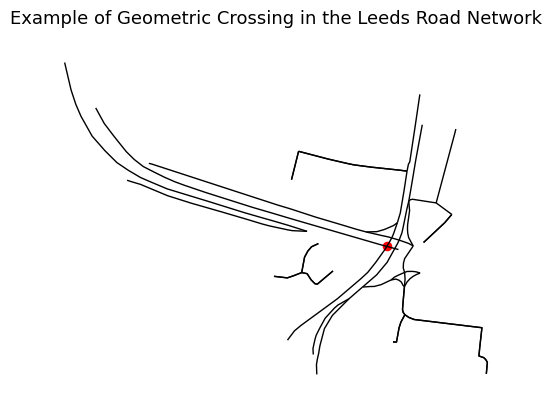
\includegraphics[width=0.47\textwidth]{figures/taskA_planarity_crossings.png}
    \caption{Illustrative geometric crossings in the selected Leeds road network. These examples support the conclusion that the network is non-planar in practice as well as in graph-theoretic form.}
    \label{fig:taskA_planarity}
    \vspace{-10pt}
\end{wrapfigure}
Planarity is tested on the simplified undirected graph, which abstracts directional and multi-edge properties. Planarity of the selected road network was tested through two approaches. The first was a graph theoretical approach where a test was performed on an undirected form of the graph representing the road network. The result was \texttt{False}, which indicates that the graph is not planar. In graph theory, a graph is defined to be planar if it can be embedded in the plane without edge-crossings \cite{lipschutz2009discrete}. Alternatively, a graph is planar if it contains neither $K_5$ nor $K_{3,3}$ as a minor. Therefore, this result confirms that the extracted road network cannot be drawn without edge-crossings while keeping the adjacency of nodes intact.
The second approach for evaluating planarity was checking the presence of any geometrical crossing in the mapped road geometry. Several examples of such crossings could be observed. One of those examples is illustrated in Fig.~\ref{fig:taskA_planarity}. The occurrence of this non-planar characteristic agrees with the discussion in the module about the reality of street networks not being planar in space since roadways can intersect through grade separations like flyovers without actually being at-grade intersections \cite{boeing2018planarity}. Thus, the non-planarity here is not only a graph-theoretic result but also a realistic property of the road system itself.\\
It can therefore be concluded that the chosen road network of Leeds is not a planar network. The importance of this statement lies in the fact that it is not always possible to assume that all crossings seen visually represent intersections for road network analysis. It can also be pointed out as one of the major differences between planar networks on paper and practical transport networks. Another drawback of this analysis can be the limited size of the chosen network, which is 1 km$^2$, so some boundary effects may occur where roads continue beyond the selected region; this is a standard issue in spatial network analysis \cite{okabe2000spatial}. Additional geometric crossing locations supporting this conclusion are provided in Appendix~\ref{appendix:part2taskA_q4}.

\subsection{\LARGE{Task B: Road Accidents}}
\leavevmode \par \noindent
This task investigates road accidents as events occurring on a spatial road network rather than as independent planar points. In line with the module content, roads are represented as edges, intersections as nodes, and distances are measured along the network rather than in Euclidean space \cite{okabe2000spatial,adams2012context}. Following this, the task is based on the network created in Task A and applies the data on the accidents observed in the time period between 2014 and 2016. The tasks that will be solved within the scope of the current task include:(i) visualise the spatial distribution of accidents on the network,  (ii) checking whether the accident-prone streets are linked to each other through the concept of spatial autocorrelation and the use of network point patterns, and (iii) whether accidents tend to happen close to road junctions or on stretches of road. The full implementation is provided in the accompanying repository \githublink{https://github.kcl.ac.uk/k25038453/network-data-analysis-coursework/blob/main/notebooks/part\_2/taskB.ipynb}.

\begin{wrapfigure}{r}{0.45\textwidth}
    \centering
    \vspace{-10pt}
    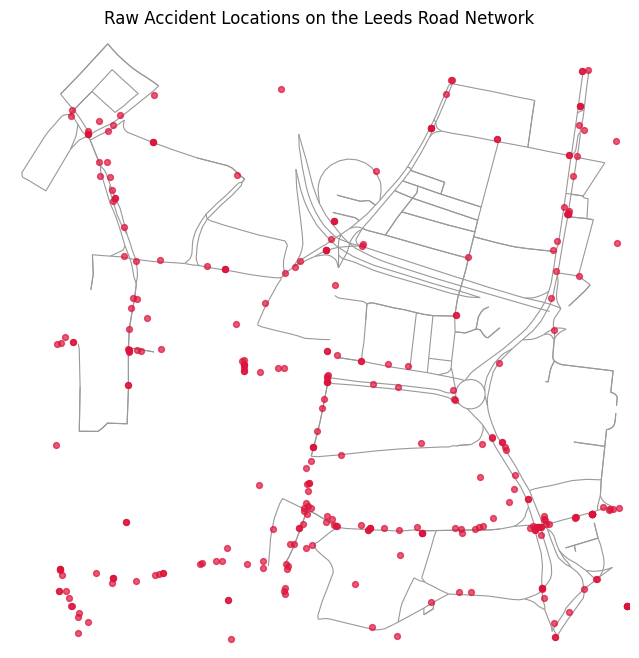
\includegraphics[width=0.45\textwidth]{figures/part2taskB_raw_accidents.png}
    \caption{Distribution of accident locations on the Leeds road network (2014--2016).}
    \label{fig:taskB_raw_accidents}
    \vspace{-10pt}
\end{wrapfigure}

\subsubsection{\large\textbf{{"Plot the distribution of road accidents on your road network and visualise this. Aggregate across multiple years of accident data. You do not need to consider or represent when the accidents happened, only their location; but you are welcome to add information about time if you believe something is interesting to show."}}}
\leavevmode \par \noindent


The data on road accidents for 2014--2016 were compiled and filtered according to the study area specified in Task A.
Figure~\ref{fig:taskB_raw_accidents} represents the spatial pattern of the accident sites on the road network. The accidents are not randomly scattered but cluster around specific sections of the road network as well as junctions.
To make sure that the analysis is in accordance with network-based activity, the accident points were snapped to the closest road networks as well. The snapping of points to road networks is explained in detail in Appendix \ref{appendix:part2taskB_q1}. This technique is consistent with the network point-pattern approach, where incidents are treated as being located on the edges \cite{okabe2000spatial}. The spaghetti library was used to explicitly represent accidents as network events, which aligns with the module’s treatment of point patterns on networks. However, for Moran’s I and the K-function, standard implementations were used to maintain clarity and control over the analytical process.


\subsubsection{\large\textbf{{" Investigate whether a high number of accidents on one road correlates with a high number on connecting roads. Calculate the k-function and the Moran's I values for
the above spatial graph. What inferences can you draw from this analysis?"}}}
\leavevmode \par \noindent

\begin{wrapfigure}{r}{0.45\textwidth}
    \centering
    \vspace{-10pt}
    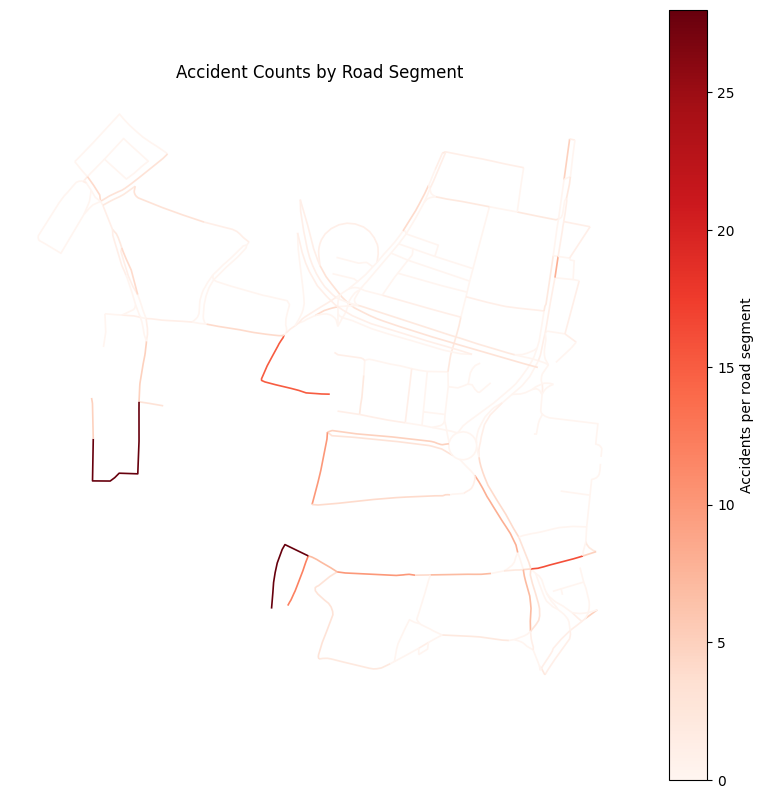
\includegraphics[width=0.48\textwidth]{figures/part2taskB_edge_accidents.png}
    \caption{Accident counts per road segment in the study area.}
    \label{fig:taskB_edge_accidents}
    \vspace{-10pt}
\end{wrapfigure}

In order to determine if the roads that have high accident frequencies connect, first the accidents had to be snapped to the network to determine how many accidents occurred on each road section, providing an edge-based approach for spatial networks.

It can be seen from Figure~\ref{fig:taskB_edge_accidents} that accident numbers are not evenly distributed within the network, but rather have certain parts where they are more concentrated.
To quantify this, Moran’s I was computed using edge adjacency (roads sharing a node). Moran’s I measures spatial autocorrelation, where positive values indicate that neighbouring edges tend to have similar accident counts \cite{adams2012context}. The computed value was positive and statistically significant (see Appendix~\ref{appendix:part2taskB_q2}), indicating that accident-prone roads tend to be connected to other accident-prone roads.
The network K-function was applied to further investigate clustering at various levels by using network distance instead of planar distances. This differs from the planar K-function in that it takes into account the network distance as well as total edge length as the spatial extent of analysis \cite{okabe2000spatial}. The results show that the K function value exceeds  the simulated CSR envelope at short distances (Appendix~\ref{appendix:part2taskB_q2}), indicating clustering of accidents along connected road segments. Moran's I and network K-function results demonstrate consistent findings suggesting that accidents do not occur randomly but rather cluster both locally (within adjacent roads) and network-wise.


\subsubsection{\large\textbf{{" Investigate whether accidents happen nearer to intersections or partway along roads. Consider this as  asking at what fraction of the road length away from the nearest intersection do accidents typically occur."}}}
\leavevmode \par \noindent
\begin{wrapfigure}{l}{0.45\textwidth}
    \centering
    \vspace{-10pt}
    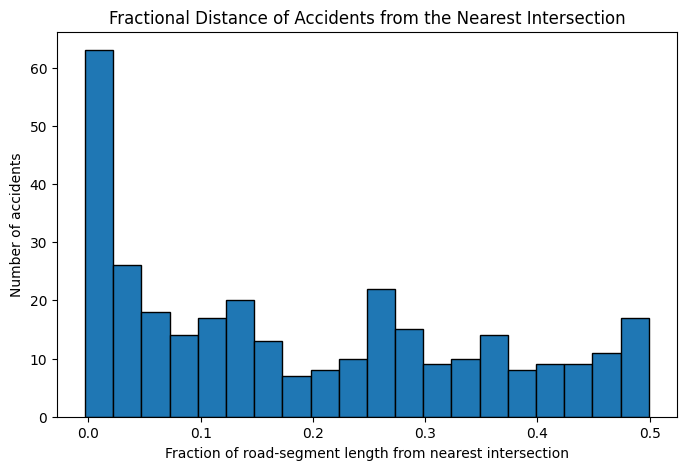
\includegraphics[width=0.465\textwidth]{figures/part2taskB_intersection_hist.png}
    \caption{Distribution of accident positions relative to the nearest intersection.}
    \label{fig:taskB_intersection_hist}
    \vspace{-10pt}
\end{wrapfigure}

To find out if the accidents happened near an intersection or on a road segment, each snapped accident was converted into the fractional distance along that specific road segment. The distance between the accident point and the nearest intersection was determined by computing the minimum value of $\min(f, 1-f)$, where $f$ was the fractional distance.
As depicted in Figure~\ref{fig:taskB_intersection_hist}, the distribution is skewed towards lower values, which indicates that a large proportion of accidents occur closer to intersections than to mid-segment locations.
This is further supported by summary statistics and threshold-based proportions (Appendix~\ref{appendix:part2taskB_q3}), which show that a substantial share of accidents occur within a small fraction of the road length from the nearest intersection.
The finding is in line with the assumption that intersections are riskier locations because of high levels of interaction between vehicles, turning manoeuvres, and complex decisions, all of which are known to be involved in accidents \cite{okabe2000spatial}.

\subsection{\LARGE{Task C: Voronoi Diagrams}}
\leavevmode \par \noindent
In this task, we use the concept of spatial network partitioning to help plan various marathon routes simultaneously in Leeds. As per the task objectives, based on the road network created for Task A and the accidents identified in Task B, our goal is to break down the city into partitions or cells where each cell can facilitate the creation of marathon routes of about 42 km. Based on the module content related to spatial partitioning and network-based Voronoi diagrams, the city will be partitioned using seed points where the distance will be computed on the road network and not Euclidean space \cite{okabe2000spatial}. The implementation is provided in the accompanying repository \githublink{https://github.kcl.ac.uk/k25038453/network-data-analysis-coursework/blob/main/notebooks/part\_2/taskB.ipynb}.

\subsubsection{\large\textbf{{"Select the initial set of 4 cell seed points. For this, you can use several criteria, such as being far away from frequent accident roads, being close to public transport, being evenly spread, etc. (explain your choice in the report)"}}}
\leavevmode \par \noindent
\begin{wrapfigure}{r}{0.45\textwidth}
    \centering
    \vspace{-10pt}
    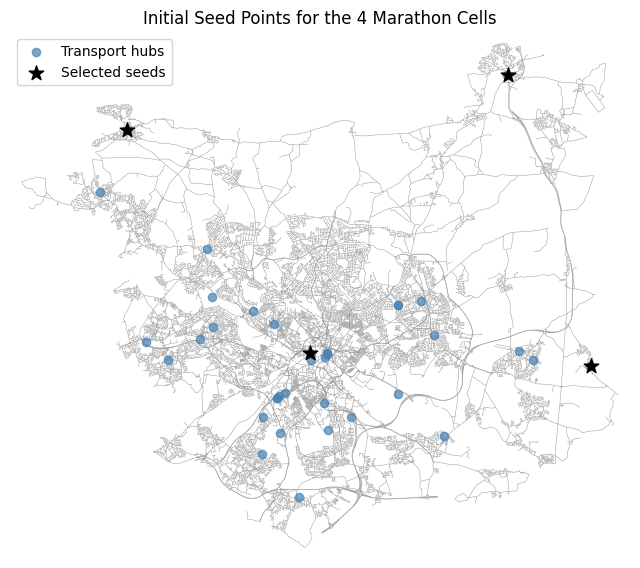
\includegraphics[width=0.415\textwidth]{figures/part2taskC_seeds.png}
    \caption{Initial seed points selected for the four marathon cells in Leeds.}
    \label{fig:taskC_seeds}
    \vspace{-10pt}
\end{wrapfigure}
Instead of just picking them at random, the first four seed points were chosen based on a mix of practical and network-based criteria. The goal was to get seeds that could work as marathon starting points and also make a balanced city-wide partition. Three things helped us choose.\\
 First, the seeds were picked so that they were spatially spread across Leeds. This was important because the mayor wants to set up marathons in different parts of the city so that people can go to one that is close to where they live. If the seeds were all in one part of the city, the Voronoi cells would be uneven and wouldn't help with that goal.\\
Second, the seeds were picked because they were near major public transportation hubs. For marathon events to work, participants and organisers need to be able to easily get to the starting line. Nodes close to major train or bus stations are better starting points than isolated network points. This criterion also makes sure that the chosen marathon sites are not only spread out geometrically but also easy to get to.\\
Third, the seed selection was made to align with the accident patterns identified in Task B. Task B showed that accidents didn't happen evenly throughout the network; instead, they happened more often on certain roads and at certain junctions. So, when picking candidate starting areas, they chose places that didn't put the partition around the accident-prone corridors. This does not imply that seeds were chosen solely by minimising accidents; rather, accident structure was utilised as a planning criterion alongside accessibility and dispersion.\\
In terms of operations, candidate seed nodes were first made from public transportation features. Then, a greedy farthest-point strategy was used to pick four nodes that were far apart from each other. This created a group of seeds that were easy to get to and spread out across the city. Figure \ref{fig:taskC_seeds} shows the chosen seed points, and further supporting details for the seed-selection process are provided in Appendix~\ref{appendix:part2taskC_seeds}

\subsubsection{\large\textbf{{"Visualise the cells yielded by our selection of seed points in a Voronoi diagram. What kind of Voronoi diagram (edge planar, node network, or edge points network) is most useful for this problem, and why?"}}}
\leavevmode \par \noindent
Using the four chosen seed points, a shortest-path Voronoi construction divided the Leeds road network into four cells. Figure~\ref{fig:taskC_voronoi} shows the cells that were made. In each cell, there is a list of network locations that are closest to one of the four seed points in terms of network distance.
Three Voronoi ideas can be used to solve this problem. An edge-planar Voronoi diagram divides regular planar space based on Euclidean distance. This is helpful for a lot of spatial problems, but it's not the best fit here because marathon accessibility depends on how well you can move through the road network, not how well you can move straight across space.\\
A node-network Voronoi diagram splits the graph by giving each node to the closest seed based on the shortest path distance along the network. This is better than the planar case because it takes into account the real road structure and how easy it is to get to the route. But it only divides the set of nodes directly.\\
An edge-point network Voronoi diagram is the best type of diagram for this job because people can start their trip from anywhere along the road network, not just from graph nodes. In that sense, the most natural way to understand "closest marathon" is that it means closeness for all points on streets, not just intersections. This is also the Voronoi type that is most closely related to urban accessibility through networks.
\begin{wrapfigure}{r}{0.45\textwidth}
    \vspace{-10pt}
    \centering
    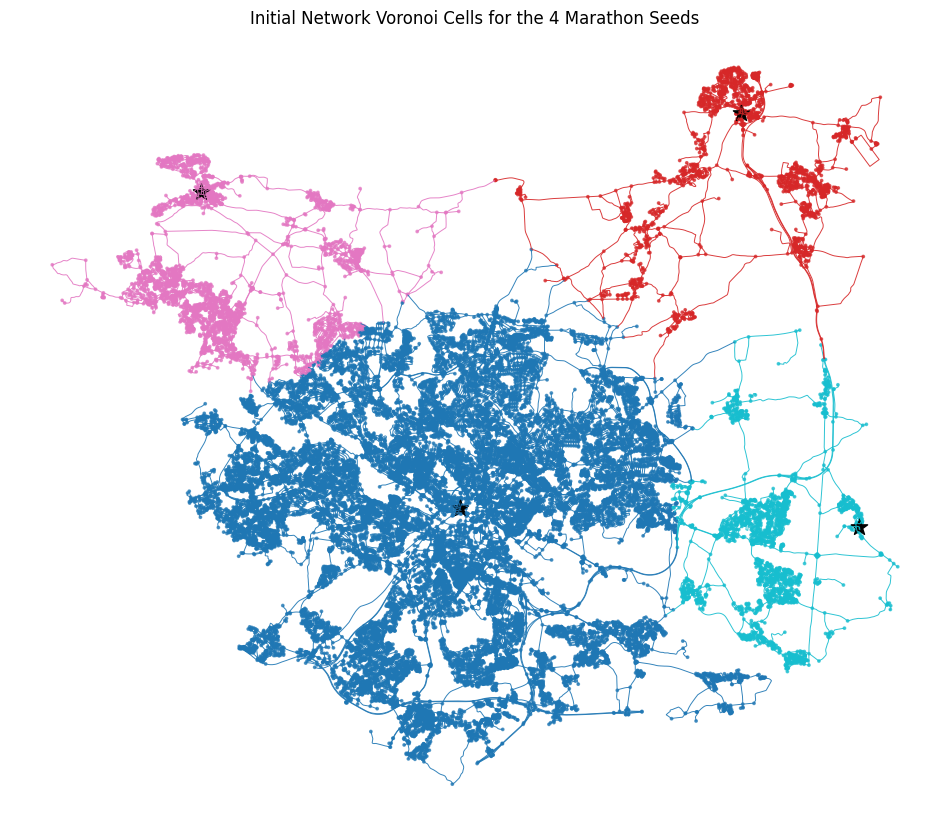
\includegraphics[width=0.475\textwidth]{figures/part2taskC_voronoi.png}
    \caption{Voronoi partition of the Leeds road network into four marathon cells.}
    \label{fig:taskC_voronoi}
    \vspace{-10pt}
\end{wrapfigure}
A real edge-points network Voronoi, on the other hand, would need to break edges into smaller pieces, like lixels, so that road segments can be split exactly between competing seeds \cite{ai2015voronoi}. This study did not utilise a complete lixel-based edge-points implementation. Instead, a weighted node-network Voronoi with edge assignment was made as a practical approximation. Nodes were assigned based on the shortest path distance, and edges were then linked to the nearest seed using the midpoint-based network distance. So, the best Voronoi idea for the planning problem is the edge-points network Voronoi. However, the solution that was put into place should be seen as a practical approximation of that idea, not a full edge-point construction. This option is still the best one because it keeps the main idea of the task, which is to divide the road system based on how easy it is to get around the network. Figure~\ref{fig:taskC_voronoi} shows the Voronoi cells that were made, and Appendix~\ref{appendix:part2taskC_voronoi} has more information.

\subsubsection{\large\textbf{{"Find 2 or 3 cells for which you can find at least one path (or more, if possible) that is (a) approximately 42 km long, and (b) finishes at the same point where it starts. Visualise both the cells and the found paths. "}}}
\leavevmode \par \noindent
The next step after building the four Voronoi cells was to find out if any of the cells had marathon routes. For each cell, the road subnetwork that went with it was taken out and searched for closed routes. For a route to be valid, it had to meet two requirements: it had to be a "closed loop," which means it started and ended at the same node, and it had to be about 42 km long. \\
The task says that the path is exactly 42 km long, but this is not always possible on a discrete weighted road network because the lengths of available road segments limit the lengths of routes. Thus, routes are treated as approximately 42 km within a small tolerance (e.g., ±1 km), rather than requiring an exact length of 42,000 metres. This is because of the discrete nature of the edge lengths of the network representation. This is a practical result of using a graph with edges that are always the same length. It's more realistic than saying that a circuit of exactly 42,000 m must always exist.
%\vspace{-4mm}
\begin{figure}[htbp]
    \centering
    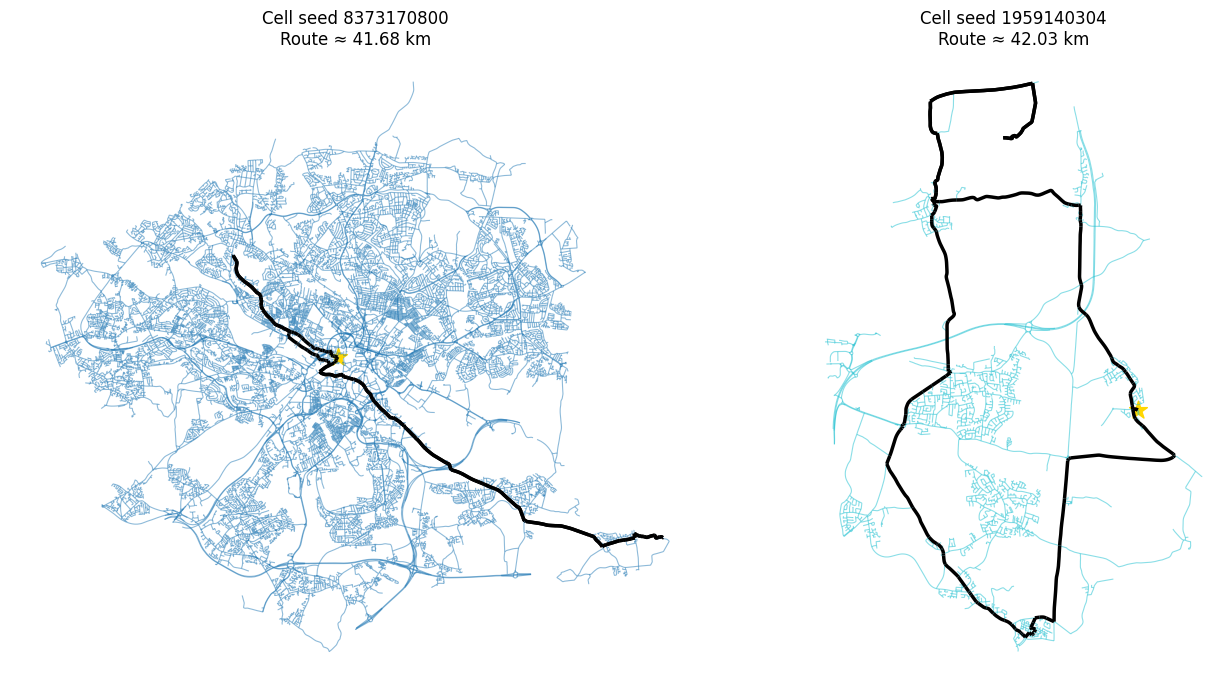
\includegraphics[width=0.6\textwidth]{figures/part2taskC_routes.png}
    \caption{Examples of approximately 42 km closed marathon routes within selected Voronoi cells.}
    \label{fig:taskC_routes}
\end{figure}
Instead of a full optimisation algorithm, a heuristic closed-route construction was used. In each cell, candidate start and intermediate nodes were chosen, and closed routes were made by putting together the shortest paths between the chosen points. This method was chosen because it is clear, can be repeated, and is good enough to find possible marathon routes without making too many claims about their bestness. Using this method, it was possible to find closed routes of about 42 km for 2–3 cells. Figure~\ref{fig:taskC_routes} shows some of these routes as examples. These visualisations directly fulfil the coursework requirement by displaying both the Voronoi cells and their corresponding route geometries. Appendix~\ref{appendix:part2taskC_routes} provides a representative route example from the alternative configuration.

\subsubsection{\large\textbf{{"Try to extend the previous step to all cells. Can you find at least one such path for every cell? "}}}
\leavevmode \par \noindent
\begin{wraptable}{r}{0.43\textwidth}
\centering
\vspace{-10pt}
\caption{Feasibility of approximately 42 km closed routes across the four initial Voronoi cells.}
\label{tab:taskC_feasibility}

\begin{tabular}{p{1.6cm} p{1.15cm} p{1.15cm} p{1.15cm}}
\toprule
\textbf{Cell} & 
\textbf{Closed route found} & 
\textbf{Within tolerance} & 
\textbf{Route length (km)} \\
\midrule
Initial cell 1 & True & True & 41.681 \\
Initial cell 2 & True & False & 35.176 \\
Initial cell 3 & True & False & 36.023 \\
Initial cell 4 & True & True & 42.032 \\
\bottomrule
\end{tabular}

\vspace{-10pt}
\end{wraptable}
The route-search process was then expanded from the chosen example cells to encompass all four initial Voronoi cells. The goal of this step was to see if the first four-seed partition makes a marathon route that works in every part of the city.
The findings indicated that this was \textit{not} the case. Only two of the four initial cells had closed routes that were about 42 km long and could be used. The other two cells didn't have subnetworks that were long enough and well-connected enough to support that route with the search strategy that was chosen. Table~\ref{tab:taskC_feasibility} shows a summary of these results, and Appendix~\ref{appendix:part2taskC_allcells} gives more information.
This result is significant as it demonstrates that a network partition deemed reasonable from an accessibility standpoint does not inherently ensure route feasibility. This means that spatial coverage and route-support capability are related goals, but they are not the same.



\subsubsection{\large\textbf{{"If for steps 3-4 there were cells with no such path, what different options could you consider to increase the number of cells that include such paths? (Hint: think about the number and location of seed points; the size of the area under consideration; etc.) Choose one of such options, repeat steps 3-4, and report the results you obtain, explaining your reasoning."}}}
\leavevmode \par \noindent
Since only 2 of the 4 initial cells had marathon routes that could work, an improvement step was needed. There are a few things that could be done to get more cells that are good for routes:\\
- changing the "location of seed points" to make cells more balanced in terms of network structure;\\ - changing the "number of seed points" to change the number and size of cells;\\ - changing the "overall study area" to allow larger or more connected subnetworks within each cell.\\
In this project, the decision was made to change the location of the seed points while keeping the number of marathons at $N=4$, as the task required. This was chosen because it is the most direct and controlled way to make the route more feasible without changing the basic planning problem. The idea was that the first seed configuration put a lot of emphasis on making it easy to get to transportation hubs. However, this may have led to cells that were not evenly able to support long closed routes. So, a seed configuration that was more evenly spread was tested to make cells that were more balanced.
After that, the Voronoi partition and route search were redone with the new seed set. The Table~\ref{tab:taskC_comparison} shows:
\begin{wraptable}{r}{0.5\textwidth}
\centering
\vspace{-10pt}
\caption{Comparison of feasible cells before and after revising the seed locations.}
\label{tab:taskC_comparison}
\begin{tabular}{p{4.5cm} p{2cm}}
\toprule
\textbf{Configuration} & 
\textbf{Feasible cells out of 4} \\
\midrule
Initial (transport + spread) & 2 \\
Alternative (pure spatial spread) & 1 \\
\bottomrule
\end{tabular}
\vspace{-10pt}
\end{wraptable}
The differences between the first and second configurations. The alternative seed configuration did not improve feasibility; instead, it reduced the number of feasible cells from two to one. This shows that just improving spatial balance doesn't make a route feasible; the internal network structure is also very important.
Appendix~\ref{appendix:part2taskC_comparison} has more information about the figures and routes.
This finding underscores a crucial planning principle: in a network-based partitioning problem, a cell's quality is influenced not solely by its area or centrality, but also by the internal configuration of its road subnetwork. So, picking seed points in a way that takes the network into account can make the partition much more useful in real life.\\


% =================================================
% REFERENCES
% =================================================
\bibliographystyle{ACM-Reference-Format}
\bibliography{references}

% =================================================
% APPENDIX
% =================================================

\newpage

\appendix

\section{Appendix A}
\label{appendix:visuals}

\subsection{Network Visualisations}
\label{appendix:A.1}
\begin{figure}[H]
\centering
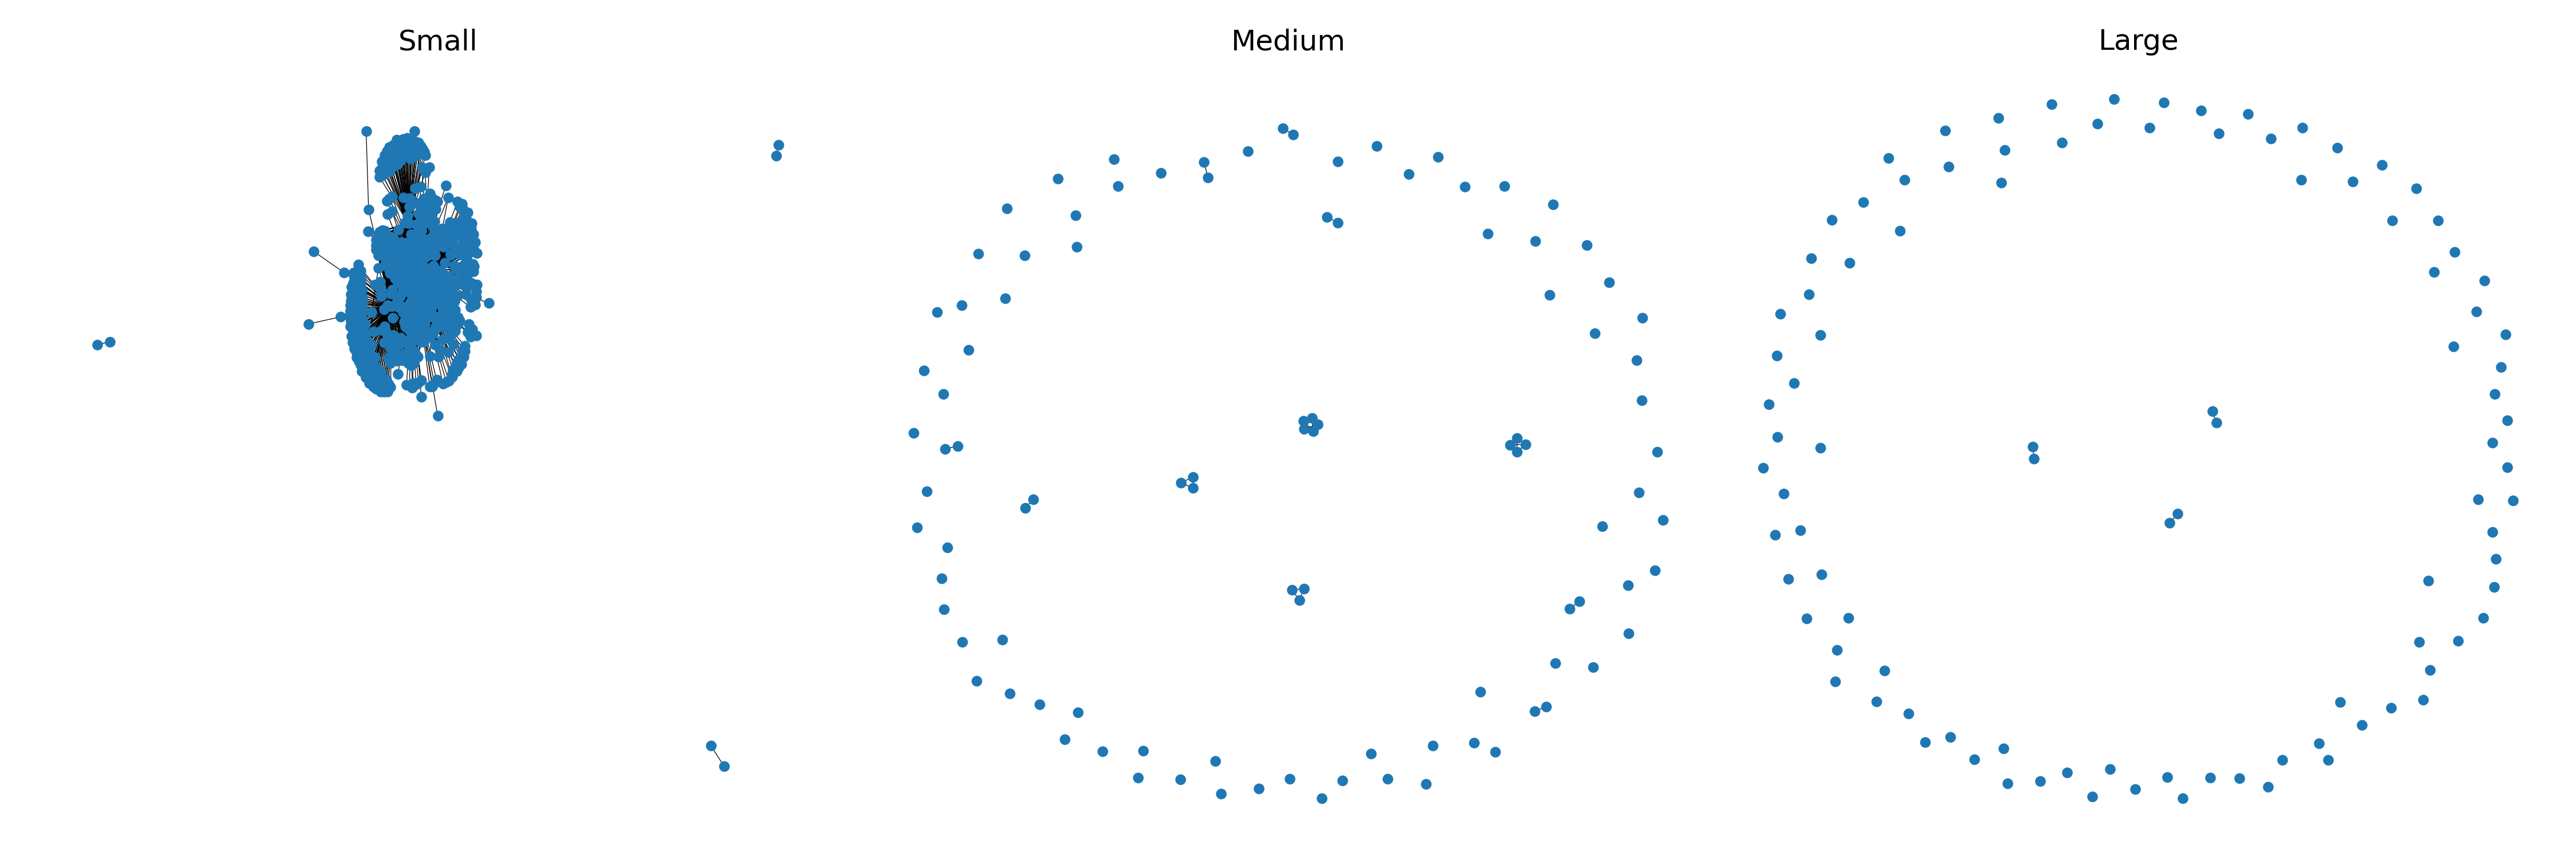
\includegraphics[width=0.9\linewidth]{figures/networks.png}
\caption{Visual representations of the three Wikidata editor networks. 
Top: Small dataset (full network). 
Middle: Medium dataset (sampled subgraph of the largest connected component). 
Bottom: Large dataset (sampled subgraph of the largest connected component).}
\label{fig:networks}
\end{figure}

\subsection{Network Summary Statistics}
\label{appendix:A.2}
\begin{table}[H]
\centering
\caption{Summary statistics of the constructed networks}
\label{tab:summary}
\begin{tabular}{lcccc}
\toprule
Dataset & Nodes & Edges & Density & Connected Components \\
\midrule
Small & 671 & 1884 & 0.00838 & 4 \\
Medium & 8396 & 24755 & 0.000702 & 264 \\
Large & 9887 & 33497 & 0.000685 & 9 \\
\bottomrule
\end{tabular}
\end{table}


\section{Appendix B: Task B — Network Metrics and Visualisations}
\label{appendix:taskB}

\subsection{Basic Structural Metrics}
\label{appendix:B.1}
\label{appendix:taskB_basic}
\begin{table}[H]
\centering
\caption{Basic structural properties of the Wikidata editor networks}
\begin{tabular}{lcccccc}
\toprule
Dataset & Nodes & Edges & Density & Avg Degree & Clustering & Largest CC \\
\midrule
Small  & 671  & 1884  & 0.008381 & 5.615 & 0.5335 & 665 \\
Medium & 8396 & 24755 & 0.000702 & 5.897 & 0.2487 & 7774 \\
Large  & 9887 & 33497 & 0.000685 & 6.776 & 0.3939 & 9870 \\
\bottomrule
\end{tabular}
\end{table}

It is clear from the results that the three networks are sparse due to their low density values that tend to decrease with increasing network size. Despite this, the average degree remains relatively stable, suggesting consistent interaction patterns across datasets. \\
The clustering coefficients are significantly high, implying highly connected groups of users in each discussion.  Moreover, there exists one major largest connected component in all three networks, signifying that the vast majority of users exist in one single connected sub-network.

\subsection{Path-Based Metrics}
\label{appendix:taskB_path}
\label{appendix:B.2}
\begin{table}[H]
\centering
\caption{Path-based metrics computed on the largest connected component}
\begin{tabular}{lcc}
\toprule
Dataset & Avg Path Length & Diameter \\
\midrule
Small  & 2.5116 & 5 \\
Medium & 3.6358 & 10 \\
Large  & 2.7020 & 6 \\
\bottomrule
\end{tabular}
\end{table}

The average path lengths are relatively small across all datasets, indicating that users are connected through short paths within the network.  The diameter is also fairly small, implying that even the two farthest points are only a few degrees apart from each other.\\
In terms of the difference between the medium network and the large network, we note that there is a larger diameter and path length in the medium network as a result of its fragmentation. Overall, these results indicate efficient connectivity within the largest connected component.

\subsection{Comparison with Random Networks}
\label{appendix:taskB_random}
\label{appendix:B.3}
\begin{table}[H]
\centering
\caption{Comparison between real networks and Erdős--Rényi random graphs}
\begin{tabular}{lcccc}
\toprule
Dataset & Real Clustering & Random Clustering & Real Path & Random Path \\
\midrule
Small  & 0.5335 & 0.0083 & 2.5223 & 3.9264 \\
Medium & 0.2487 & 0.0006 & 3.6435 & 5.2824 \\
Large  & 0.3939 & 0.0007 & 2.7008 & 5.0174 \\
\bottomrule
\end{tabular}
\end{table}

As evident from the analysis above, the real networks have significantly higher clustering coefficients than their corresponding random graphs, indicating strong local structure. In contrast, random graphs exhibit near-zero clustering due to independent edge formation.\\
Although both the real and the random network types possess relatively short path lengths between each pair of edges, only the real networks feature the combination of short path lengths and high clustering, which represents the key attribute of small-world networks.

\subsection{Degree Distribution}
\label{appendix:degree_distribution}
\label{appendix:taskB_figures}
\label{appendix:B.4}
\begin{figure}[H]
\centering
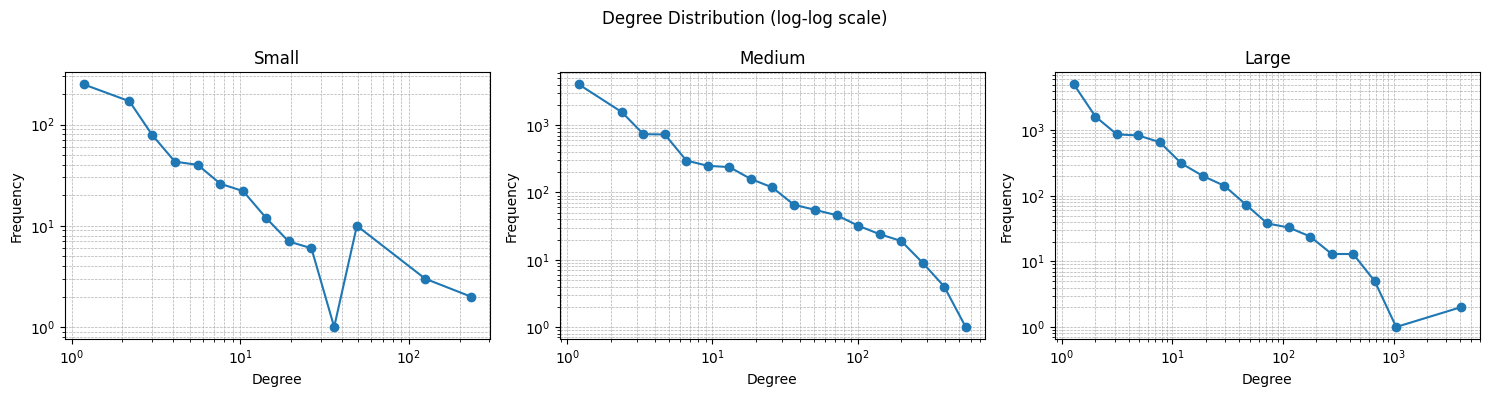
\includegraphics[width=\linewidth]{figures/degree_distributions.png}
\caption{Degree distributions of the three networks plotted on a log--log scale}
\end{figure}

The degree distributions exhibit a heavy-tailed pattern across all datasets. Most nodes have low degree, while a small number of nodes have significantly higher connectivity.\\
It shows that there exist hub nodes, which help maintain connectivity across nodes in the network. Such patterns are commonly observed in real-world social and communication networks, where interaction is unevenly distributed among participants.


\section{Appendix C: Task C — Epoidemic Models\& Prioritisation Results}
\label{appendix:taskC}

\subsection{Non-Propagation Plausibility}
\label{appendix:taskC_plausibility}
\label{appendix:C.1}
\begin{table}[H]
\centering
\caption{Local structural indicators used to assess non-propagation plausibility}
\begin{tabular}{lcccc}
\toprule
Dataset & Seed Count & Immediate Neighbours & Two-Hop Editors & Avg Shared-Neighbour Score \\
\midrule
Small  & 2 & 80 & 567 & 16.33 \\
Medium & 2 & 15 & 930 & 1.60 \\
Large  & 2 & 38 & 9035 & 17.71 \\
\bottomrule
\end{tabular}
\end{table}

The findings indicate that the large and small networks exhibit a relatively high degree of structural exposure in the presence of suspicious editors compared to the medium-sized network. The study reveals that there exists more structural plausibility in propagating information in the large and small networks.


\subsection{Priority Ranking and Seed Comparison}
\label{appendix:taskC_priority}
\label{appendix:C.2}
\begin{table}[H]
\centering
\caption{Top-ranked editors based on combined prioritisation score (small dataset)}
\begin{tabular}{lccccc}
\toprule
Node & Distance  & Neighbour & Simulation & Combined & Priority \\
 & Rank & Rank & Rank & Score & Rank \\
\midrule
Jura1 & 3 & 2 & 1 & 6 & 1 \\
Tagishsimon & 4 & 1 & 2 & 7 & 2 \\
Larske & 5 & 6 & 3 & 14 & 3 \\
Dipsacus fullonum & 7 & 5 & 4 & 16 & 4 \\
Matěj Suchánek & 8 & 4 & 5 & 17 & 5 \\
\bottomrule
\end{tabular}
\end{table}

This ranking shows that those editors who were selected by different approaches have received higher priority. This proves that the use of both structural and diffusion measures leads to results more reliable prioritisation strategy.


\subsection{One-Seed vs Two-Seed Comparison}
\label{appendix:taskC_seeds}
\label{appendix:C.3}

\begin{table}[H]
\centering
\caption{Propagation reach under one-seed and two-seed scenarios}
\begin{tabular}{lcccc}
\toprule
Dataset & One Seed & Mean Reached & Two Seed & Mean Reached \\
 & Count & (One Seed) & Count & (Two Seeds) \\
\midrule
Small  & 1 & 269.1 & 2 & 270.23 \\
Medium & 1 & 2461.7 & 2 & 2479.10 \\
Large  & 1 & 3850.5 & 2 & 3842.70 \\
\bottomrule
\end{tabular}
\end{table}

As seen from the findings, the use of two seed nodes enhances the spread, though it depends on the network structure. This means that two starting points play a vital role in enhancing the process of spread.


\section{Appendix D: Task A — Spatial Networks and Planarity}
\label{appendix:part2taskA}

\subsection{City-wide Accident Distribution and Study Area Selection}
\label{appendix:part2taskA_q1}

\begin{figure}[H]
    \centering
    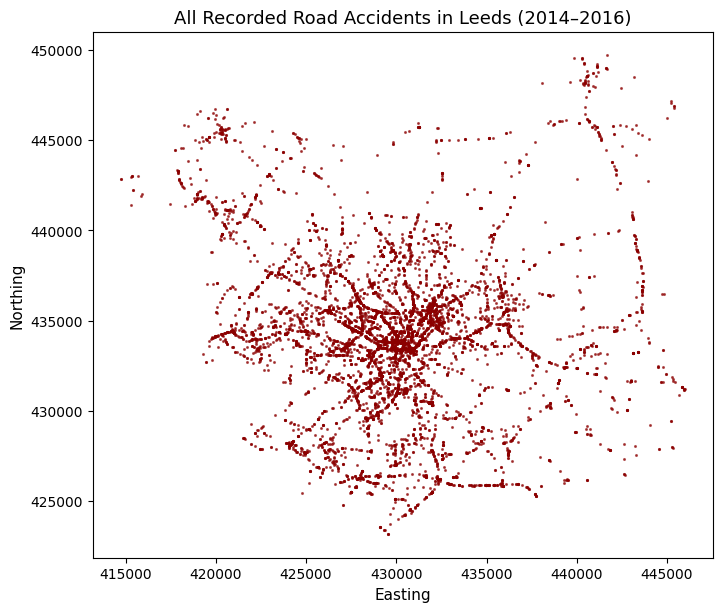
\includegraphics[width=0.6\textwidth]{figures/part2taskA_all_accidents_leeds.png}
    \caption{All recorded road accidents in Leeds (2014--2016), used to guide the central study-area selection.}
\end{figure}

This diagram depicts the spatial distribution of accidents before choosing the research area. It is quite obvious that there is a high concentration of accidents in the central part of the city, and hence, it makes sense to narrow down the search within the window of central Leeds. This way, the selected 1 km$^2$ study area will be centrally placed as well as accident-prone.

\subsection{Road Network of the Selected Study Area}
\label{appendix:part2taskA_q2}

\begin{figure}[H]
    \centering
        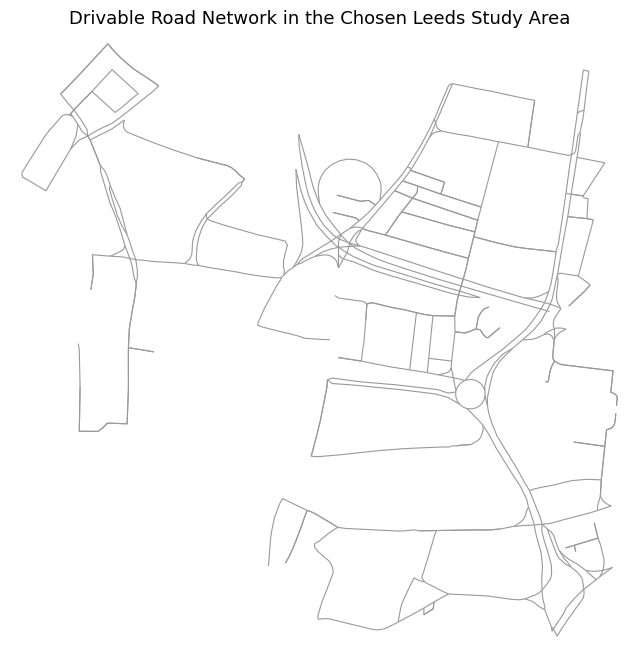
\includegraphics[width=0.5\textwidth]{figures/part2taskA_network_plot.png}
    \caption{Drivable road network extracted for the selected 1 km$^2$ study area.}
\end{figure}

The figure below presents the drivable road network employed in this study after cleaning the OpenStreetMap data set to extract drivable roads only. The network demonstrates a highly connected urban topology with short roads and intersections that are very close to one another, which is in line with the high node density observed in the main text.

\subsection{Geometric Evidence of Non-Planarity}
\label{appendix:part2taskA_q4}

\begin{figure}[H]
    \centering
    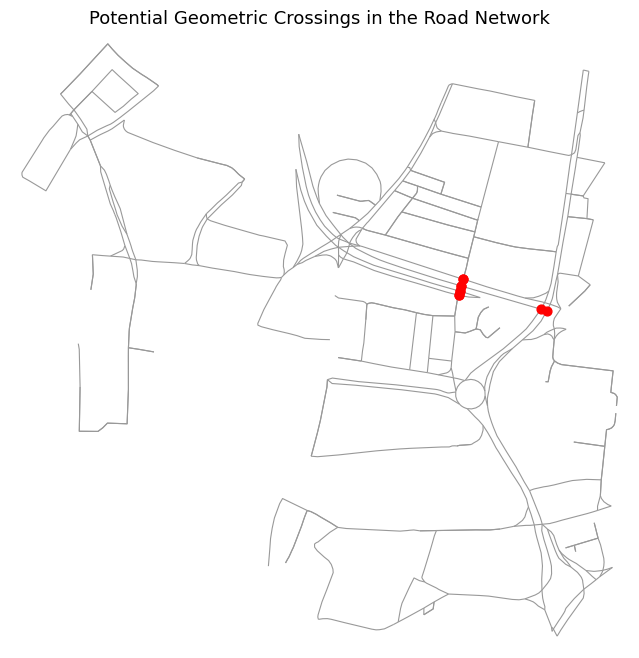
\includegraphics[width=0.45\textwidth]{figures/taskA_crossing_overview.png}
    \caption{Detected geometric crossings in the selected Leeds road network.}
\end{figure}

This diagram illustrates several places where there are crossings between road segments but no actual nodes at those intersections. The crossings result from road structures that involve grade separation (i.e., bridges or flyovers). They demonstrate that the graph is indeed non-planar. A diagram of one such crossing is presented in the report.

\section{Appendix E: Task B — Road Accidents}
\label{appendix:part2taskB}

\subsection{Accident Distribution and Network Mapping}
\label{appendix:part2taskB_q1}

\begin{figure}[H]
    \centering
    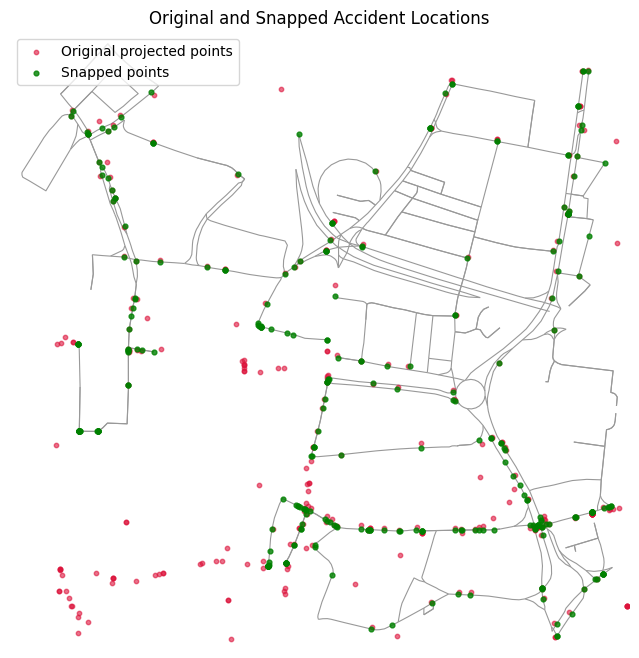
\includegraphics[width=0.48\textwidth]{figures/part2taskB_snapped_vs_original.png}
    \caption{Comparison of original accident locations and snapped network positions.}
\end{figure}

This figure shows the comparison of the original points where the accidents occurred and the locations where those points were snapped onto the road network. Snapping helps in ensuring that an accident has been associated with a road segment. It is apparent from the figure that there is a high correlation between the two points, implying that the accident points have been accurately recorded.

\subsection{Spatial Autocorrelation and Network K-function Results}
\label{appendix:part2taskB_q2}

\begin{table}[H]
\centering
\caption{Moran’s I statistics for accident counts on road segments}
\begin{tabular}{lr}
\toprule
Metric & Value \\
\midrule
Moran’s I & 0.3595879326256184 \\
Expected I under randomness &  -0.0035460992907801418 \\
p-value (permutation) & 0.001 \\
z-score & 9.330201564011523 \\
\bottomrule
\end{tabular}
\end{table}

The positive Moran's I statistic implies that road links experiencing accidents in large numbers are often linked to those experiencing accidents in equally large numbers, suggesting the presence of spatial autocorrelation within the network. The low p-value confirms that this pattern is statistically significant and unlikely to arise under spatial randomness.

\begin{figure}[H]
    \centering
    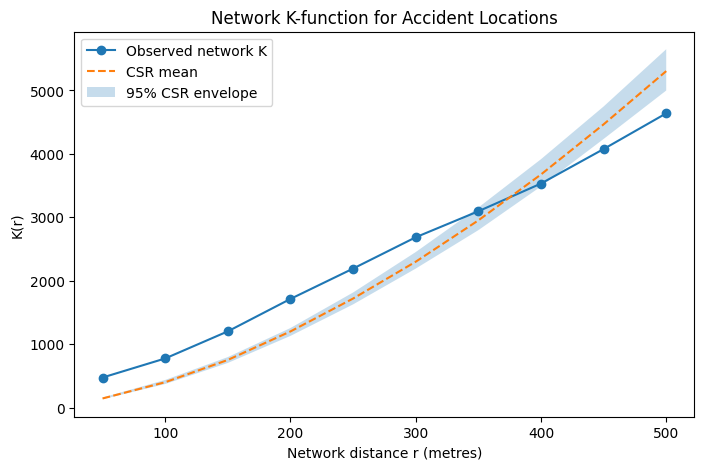
\includegraphics[width=0.55\textwidth]{figures/part2taskB_k_function.png}
    \caption{Network K-function with CSR envelope.}
\end{figure}

This graph demonstrates the relationship between the K-function for the network and the Monte Carlo CSR envelope. The graph crossing the envelope at close proximity shows that there is a cluster pattern for the occurrence of accidents on the road network. This supports the conclusion that accident locations are not randomly distributed but tend to cluster within connected parts of the network.

\subsection{Distance from Intersections Analysis}
\label{appendix:part2taskB_q3}

\begin{table}[H]
\centering
\caption{Summary statistics of accident positions relative to nearest intersections}
\begin{tabular}{lr}
\toprule
Metric & Value \\
\midrule
Mean fraction & 0.188973 \\
Median fraction & 0.152004 \\
Proportion within 10\% & 0.412500 \\
Proportion within 20\% & 0.556250 \\
Proportion within 25\% & 0.615625 \\
\bottomrule
\end{tabular}
\end{table}

From the summary statistics, it is evident that a fairly significant percentage of accidents happen within proximity to intersections. The low means and medians for the fractional distances point towards the fact that accidents tend to be more concentrated around intersections rather than being uniformly distributed along road segments.

\section{Appendix F: Task C — Voronoi Diagrams and Marathon Planning}
\label{appendix:part2taskC}

\subsection{Supporting Details for Seed Selection}
\label{appendix:part2taskC_seeds}

The main report shows the final seed points that were chosen to make the Voronoi partition. 
This appendix gives more information that helps the seed-selection process.

We first found candidate seed locations by looking at how close they were to major transport corridors and how evenly they were spread out across the study area. We chose four seed points from these candidates to balance:
\begin{itemize} 
\item spatial coverage of the network,
\item accessibility via major roads and transport links,
\item the avoidance of accident-prone areas found in Task B. \end{itemize}

These things make sure that the Voronoi cells that come out are well-distributed and good for setting up marathon routes in the city.

\vspace{5pt}
\textit{Note: During development, more exploratory seed configurations were tested, but they are not shown in the main report for clarity.}

\subsection{Alternative Voronoi Configuration}
\label{appendix:part2taskC_voronoi}

\begin{figure}[H]
    \centering
    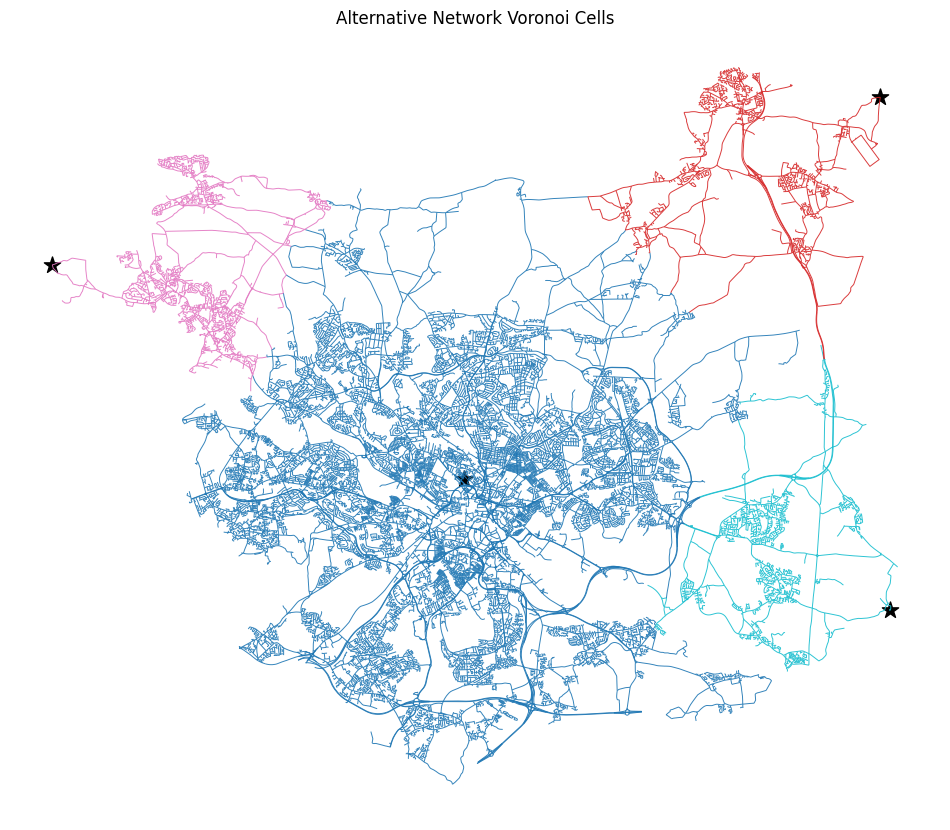
\includegraphics[width=0.8\textwidth]{figures/part2taskC_alt_voronoi.png}
    \caption{Alternative Voronoi partition obtained after revising seed locations using a purely spatial spread criterion.}
\end{figure}

This is the Voronoi partition that was made after changing the way seeds are chosen. 
This alternative, on the other hand, puts more emphasis on spatial balance across the network than on being close to transportation features. The main report talks about how this setup is different from the first one.

\subsection{Alternative Route Example}
\label{appendix:part2taskC_routes}

\begin{figure}[H]
    \centering
    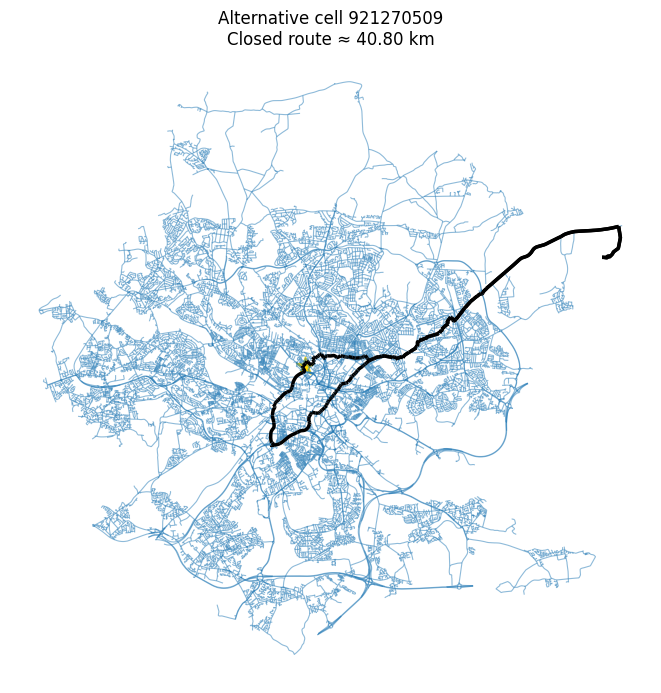
\includegraphics[width=0.8\textwidth]{figures/part2taskC_alt_route.png}
    \caption{Example of an approximately 42 km closed route identified within an alternative Voronoi cell.}
\end{figure}

This figure shows one example of a closed route that was found using the alternative seed configuration. 
The route is in the right Voronoi cell and meets the approximate 42 km requirement within the range used in the analysis.

In the first setup, only some cells could create viable routes. In the new setup, routes can be found in a different way of dividing the network into spaces. This backs up the comparison that was talked about in the main report.

\subsection{Detailed Feasibility Results for All Cells}
\label{appendix:part2taskC_allcells}

\begin{table}[H]
\centering
\caption{Detailed feasibility results for the initial Voronoi configuration.}
\begin{tabular}{lcccc}
\toprule
Cell & Nodes in cell & Edges in cell & Within tolerance & Route length (km) \\
\midrule
Initial cell 1 & 25245 & 30345 & True & 41.681 \\
Initial cell 2 & 1605 & 1829 & False & 35.176 \\
Initial cell 3 & 2771 & 3207 & False & 36.023 \\
Initial cell 4 & 1979 & 2228 & True & 42.032 \\
\bottomrule
\end{tabular}
\end{table}

This table gives more information about the structure of each Voronoi cell, such as how many nodes and edges are in each subnetwork. It adds to the summary results in the main report and backs up the idea that only some cells have good marathon routes.

\subsection{Comparison of Initial and Alternative Configurations}
\label{appendix:part2taskC_comparison}

\begin{table}[H]
\centering
\caption{Comparison of route feasibility across initial and alternative seed configurations.}
\begin{tabular}{lc}
\toprule
Configuration & Feasible cells (out of 4) \\
\midrule
Initial (transport + spread) & 2 \\
Alternative (pure spatial spread) & 1 \\
\bottomrule
\end{tabular}
\end{table}

This table shows how many Voronoi cells had a viable closed route of about 42 km for each seed configuration.

In the first setup, only two of the four cells met the route-length requirement. As a result, the alternative configuration was put into place by changing the seed-selection strategy to put more emphasis on spatial balance across the network.

The results demonstrate that the alternative configuration does not increase the number of feasible cells in this instance. This means that seed placement affects how the network is divided into different areas, but it doesn't guarantee that the routes will be better. That depends on the structure and connectivity of each cell subnetwork.

\end{document}